\subsection{Implementation}
%The process for which metrics, algorithms, and techniques were implemented with the given datasets or input data has been thoroughly documented. Complications that occurred during the coding process are discussed.


As I introduced in the section2.4(Benchmark), I utilized the 4 convolutional layers and 2 fully connected layers.In this section, I explain the architecture of the model in more depth.

The objective of the learning is to minimize the cross entropy in the learning process.
The architecture of the model is the following.

 \begin{figure}[H]

	\begin{center}
	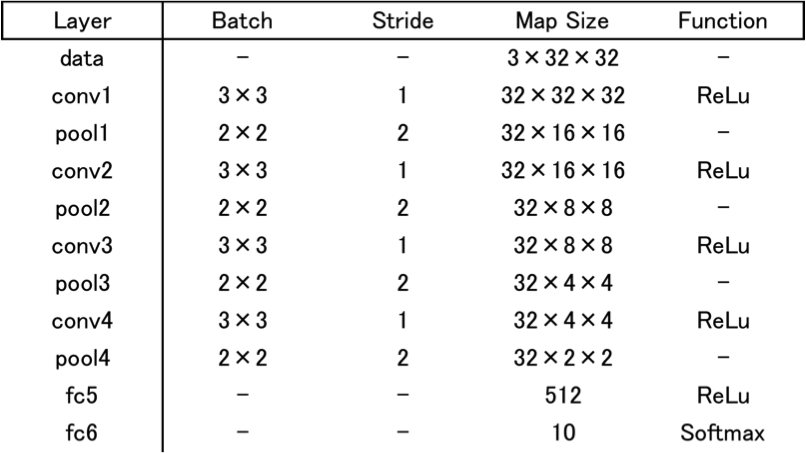
\includegraphics[width=7cm]{picture/layer_architecture.png}
	\caption{Architecture of the model}
	\end{center}
	\label{fig:9}

\end{figure}


To train the CNN model, I used Keras which is one of the neural network libraries like Theano or Tensorflow.

As for the optimizer, I utilized 'Adam'. The important parameters training the model is as follows.
Optimization parameters:Learning rate $\alpha$=0.001, $\beta_{1}$=0.9,$\beta_{2}=0.999$,$\epsilon=1.0\times10^{-8}$\cite{Adam}

Adam ,Adaptive Moment Estimation, is a online method to estimate the average and variance of the gradient. With these information, adam can update learning rate. Adam keeps not only an exponentially decaying average of the past squared gradient but also an exponentially decaying average of the past gradient.
\begin{eqnarray}
 m_{t}=\beta_{1}m_{t-1}+(1-\beta_{1})g_{t}
 \end{eqnarray}
\begin{eqnarray}
v_{t}=\beta_{2}v_{t-1}+(1-\beta_{2})g^{2}_{t}
\end{eqnarray}


$m_{t},v_{t}$ are estimates of the first moment and the second moment of the gradients.At first these values are set to be 0.
Then, $m_{t},v_{t}$ are divided by$1-\beta_{1},1-\beta_{2}$,respectively.
\begin{eqnarray}
 \hat{m_{t}}=\frac{m_{t}}{1-\beta^{t}_{1}}
 \end{eqnarray}
 \begin{eqnarray}
 \hat{v_{t}}=\frac{v_{t}}{1-\beta^{t}_{2}}
 \end{eqnarray}

Finally, by using these to update parameters, we get the formula of Adam.
 \begin{eqnarray}
 \theta_{t+1}=\theta_{t}-\frac{\alpha}{\sqrt{\hat{v_{t}}}+\epsilon}\hat{m_{t}}
 \end{eqnarray}

The number of stride or map size are shown in Fig.12.
As for the initialization of the random weights in convolutional layers, I used uniform distribution.
I used normalized uniform distribution which is proposed by Glorot\cite{Glorot} for the initialization of the weights in fully connected layers
I used ReLU(Rectified Linear Unit) as the activation except for the final layer and I used softmax as the final layer of activation.


\begin{eqnarray}
 a_{ReLU}=\log(1+\exp(x)) \simeq \max(0,x)
\end{eqnarray}


With this setting, I got the accuracy rate of 70.2\%
